


\section[Unsupervised ML]{Unsupervised machine learning}

\begin{frame}{A lot of applications and use cases, \ldots}
\ldots but we'll distinguish two today:

\begin{enumerate}
\item Finding similar variables (dimension reduction)
\item Finding similar cases (clustering)
\end{enumerate}

\pause

Are we more interested in which features ``belong together'' or which cases ``belong together''? 

\emph{There are many other techniques than those presented today, and vice versa, those presented today can also be used for other purposes}

\end{frame}

\subsection{Finding similar variables}

\subsubsection{An introduction to dimensionality reduction}

\begin{frame}{Dimensionality reduction}
dimensionality = the number of features we have



\begin{block}{(1) Explorative data analysis and visualization}
\begin{itemize}
\item No good way to visualize 10,000 dimensions (or even 4)
\end{itemize}
\end{block}

\pause


\begin{block}{(2) The curse of dimensionality}
More features means more data (good!), but:
\begin{itemize}
\item Too many features can lead to unfeasible computation times
\item We need more training cases to increase the likelihood that the possible combinations actually occur
\end{itemize}
\end{block}
\end{frame}



\begin{frame}[fragile]{Dimensionality reduction}

\begin{block}{First approach: feature selection}
\begin{itemize}
\item Only choose the features that are really relevant
\end{itemize}
\end{block}


Example: Exclude all terms that occur in more than 50\% of the documents, or in less than $n=5$ documents:

\begin{lstlisting}
vec = CountVectorizer(max_df=0.5, min_df=5)
\end{lstlisting}

\tiny{\url{https://scikit-learn.org/stable/modules/generated/sklearn.feature\_extraction.text.CountVectorizer.html}}

\end{frame}





\begin{frame}[fragile]{Dimensionality reduction}

\begin{block}{Second approach: feature extraction}
\begin{itemize}
\item Create a smaller set of features
\item E.g.: 1,000 features $\rightarrow$ PCA to reduce to 50 components $\rightarrow$ SML with these 50 component scores as features
\end{itemize}
\end{block}

\end{frame}



\begin{frame}[fragile]{Dimensionality reduction}

So, we can use unsupervised ML as a dimension reduction step in a supervised ML pipeline. 
\vspace{0.5cm}
But it can also be a goal in itself, to understand the data better or to visualize them.
\end{frame}







\subsubsection{Principal Component Analysis and Singular Value Decomposition}


\begin{frame}{PCA}
\begin{itemize}
\item related to and often confused with Factor Analysis (same menu item in SPSS -- many people who believe they run FA actually run PCA!)
\item Components are ordered (first explains most variance)
\item Components do \emph{not} necessarily carry a meaningful interpretation
\end{itemize}
\end{frame}

\begin{frame}{PCA}
\makebox[\linewidth]{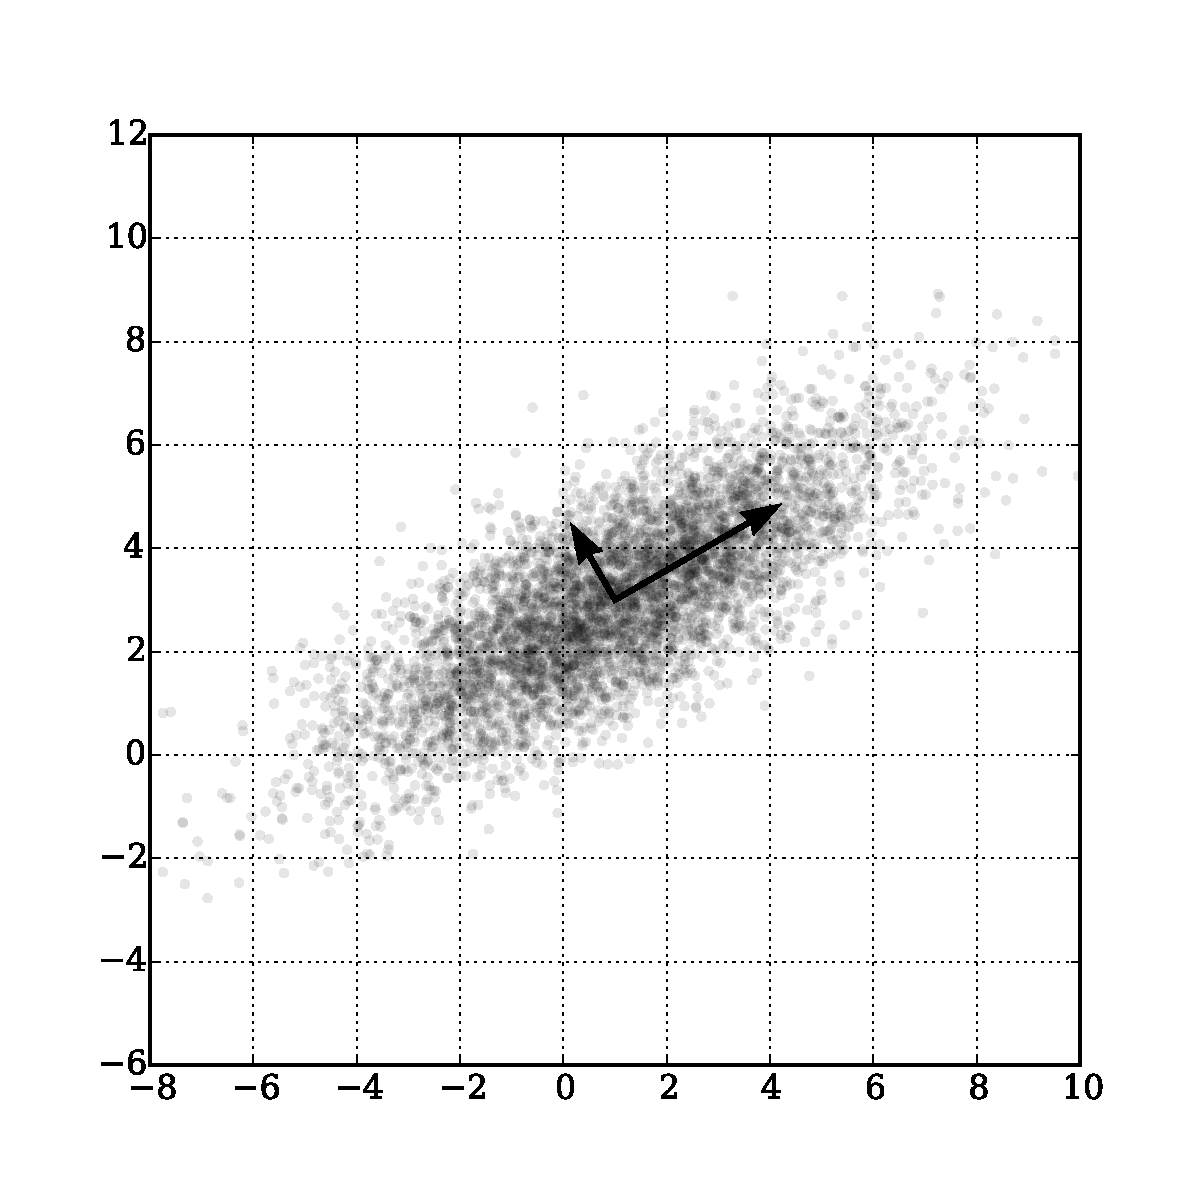
\includegraphics[width=\paperwidth,height=.6\paperheight,keepaspectratio]{pca}}

\tiny{\url{https://upload.wikimedia.org/wikipedia/commons/f/f5/GaussianScatterPCA.svg}}
\end{frame}



\begin{frame}[fragile,plain]{Preparation: Import modules and get some texts}
\begin{lstlisting}
from sklearn import datasets
from sklearn.decomposition import PCA
from sklearn.decomposition import TruncatedSVD
from sklearn.feature_extraction.text import CountVectorizer
from sklearn.pipeline import make_pipeline
from sklearn.preprocessing import FunctionTransformer
import matplotlib.pyplot as plt
%matplotlib inline

autotexts = datasets.fetch_20newsgroups('rec.autos', remove=('headers', 'footers', 'quotes'), subset='train')['data']
religiontexts = datasets.fetch_20newsgroups('soc.religion.christian', remove=('headers', 'footers', 'quotes'), subset='train')['data']

texts = autotexts[:20] + religiontexts[:20]
\end{lstlisting}
\end{frame}




\begin{frame}[fragile,plain]{Running PCA}
PCA does not accept a \textit{sparse matrix} as input (but the CountVectorizer gives one as output), so we need to transform it into a \textit{dense matrix}.

\begin{lstlisting}
myvec = CountVectorizer(texts, max_df=.5, min_df=5)
mypca = PCA(n_components=2)

mypipe = make_pipeline(myvec, FunctionTransformer(lambda x: x.todense(), accept_sparse=True), mypca)

r = mypipe.fit_transform(texts)
\end{lstlisting}
\end{frame}



\begin{frame}[fragile,plain]{Plotting the result}
\begin{lstlisting}
plt.scatter([e[0] for e in r], [e[1] for e in r], alpha=.6)
\end{lstlisting}

\makebox[\linewidth]{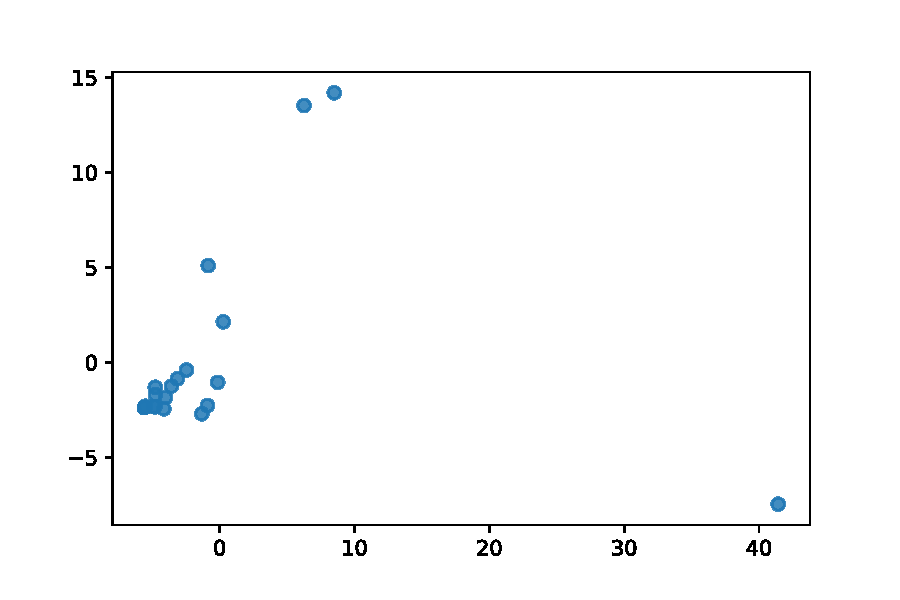
\includegraphics[width=\paperwidth,height=.6\paperheight,keepaspectratio]{pca-example}}


\end{frame}



\begin{frame}[fragile]{Singular value decomposition}
The need to use a dense matrix is \emph{really} a problem for large feature sets (which we have in NLP).
\pause

We therefore can better use SVD, which is essentially* the same and very simple to use:

\begin{lstlisting}
mysvd = TruncatedSVD(n_components=2)
mypipe = make_pipeline(myvec, mysvd)
r = mypipe.fit_transform(texts)
\end{lstlisting}

\footnotesize{(In this specific case, we even get exactly the same plot\ldots)}


\footnotesize{
* It's mathematically different, but SVD is even used ``under the hood'' by several PCA modules to solve PCA problems.

More info and background: \url{https://towardsdatascience.com/pca-and-svd-explained-with-numpy-5d13b0d2a4d8}}

\end{frame}







\subsection{Finding similar cases}

\subsubsection{k-means clustering}




\begin{frame}{Grouping features vs grouping cases}
Let's consider a corpus of several thousand user comments.

We could use SVD, MDS, or similar techniques to 
\begin{itemize}
\item figure out relationships between features
\item see which features stand out
\item get a first sense what topics are in the corpus.
\end{itemize}
\pause

But:
\begin{itemize}
\item<+-> We do not learn anything about \emph{which} texts (cases) belong to which topic
\item<+-> We could use the component scores returned by \texttt{.fit\_transform()} to then group our cases
\end{itemize}

\pause 
$\Rightarrow$ \footnotesize{Alternative: Choose the opposite approach and first find out which cases are most similar, \textit{then} describe what features characterize each group of cases}


\end{frame}




\begin{frame}{k-means clustering}
\begin{itemize}[<+->]
\item Goal: group cases into $k$ clusters
\item $k$ is set in advance
\item Algorithm to determine \textit{k} centroids (points in the middle of the cases that belong to it) such that the distances between the cases and their centroids are minimized
\item non-deterministic: starts with a randomly choosen centroids (there are other versions)
\item Cheap to compute: works even with large number of cases
\item We can run PCA first to reduce the number of features if we want/need to
\end{itemize}
\end{frame}




\begin{frame}{k-means clustering}
\makebox[\linewidth]{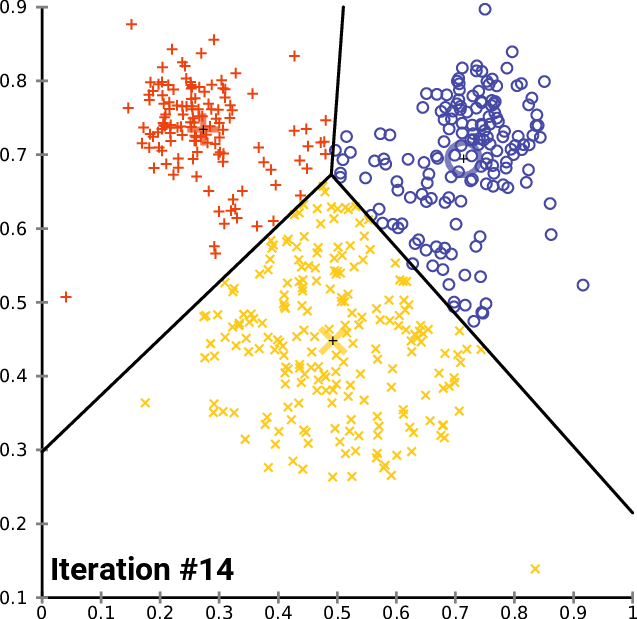
\includegraphics[width=\paperwidth,height=.65\paperheight,keepaspectratio]{kmeans}}

{\tiny{\url{https://upload.wikimedia.org/wikipedia/commons/e/ea/K-means\_convergence.gif}}}

Notice the big symbols indicating the centroids.
\end{frame}


\begin{frame}[plain,fragile]
\begin{lstlisting}
from sklearn.feature_extraction.text import TfidfVectorizer
from sklearn.cluster import KMeans

k = 5
texts = ['text1 ejkh ek ekh', 'ekyerykel'] # a list of texts

vec = TfidfVectorizer(min_df=5, max_df=.4)
features = vec.fit_transform(texts)
km = KMeans(n_clusters=k, init='k-means++', max_iter=100, n_init=1)
predictions = km.fit_predict(features)

\end{lstlisting}

That's it!
\pause

\begin{itemize}
\item \texttt{predictions} is a list of integers indicated the predicted cluster number. We can thus use \texttt{zip(predictions, texts)} to put them together.
\item<+-> We could also use \texttt{.fit()} and \texttt{.transform()} sperately and use our \texttt{km} to predict clusters for additional cases we have not used to train the model
\end{itemize}

\end{frame}


\begin{frame}[fragile,plain]{Let's get the terms closest to the centroids}
\begin{lstlisting}
order_centroids = km.cluster_centers_.argsort()[:, ::-1]
terms = vec.get_feature_names()

print("Top terms per cluster:")

for i in range(k):
    print("Cluster {}: ".format(i), end='')
for ind in order_centroids[i, :10]:
    print("{} ".format(terms[ind]), end='')
    print()
\end{lstlisting}
\pause
returns something like:

\begin{lstlisting}
Top terms per cluster:
Cluster 0: heard could if opinions info day how really just around 
Cluster 1: systems would ken pc am if as care summary ibm 
Cluster 2: year car years was my no one higher single than 
Cluster 3: which like seen 1000 few easily based personal work used 
Cluster 4: as was he if they my all will get has 
\end{lstlisting}
\end{frame}


\begin{frame}{Using k-means clustering\ldots}
\begin{itemize}
\item we get the cluster membership for each text; and
\item we get the terms that are most characteristic for the documents in each cluster.
\end{itemize}
\end{frame}

\begin{frame}{Finding the optimal $k$}

\begin{itemize}
\item The only way to find $k$ is to estimate multiple models with different $k$s
\item No single best solution; finding a balance between error within clusters (distances from centroid) and low number of clusters.
\item An elbow plot can be helpful (see example in Burscher et al, 2016)
\end{itemize}

\pause

\footnotesize 
Code-example for creating an elbow plot:
\url{https://pythonprogramminglanguage.com/kmeans-elbow-method/}

(Don't forget to insert \texttt{\%matplotlib inline} to actually see the plot)


\tiny{Burscher, B., Vliegenthart, R., \& de Vreese, C. H. (2016). Frames beyond words: Applying cluster and sentiment analysis to news coverage of the
nuclear power issue.\textit{ Social Science Computer Review, 34}(5), 530-545. doi:10.1177/0894439315596385}
\end{frame}


\subsubsection{Hierarchical clustering}

\begin{frame}{Downsides of k-means clustering}
k-means is fast, but has problems:

\begin{itemize}
\item $k$ can only be determined by fitting multiple models and comparing them
\item bad results if the wrong $k$ is chosen
\item bad results if the (real) clusters are non-spherical
\item bad results if the (real) clusters are not evenly sized
\end{itemize}
\end{frame}


\begin{frame}{Hiearchical clusttering}
\begin{block}{General idea}
\begin{itemize}
\item To start, each case has its own cluster
\item Merge the two clusters that are most similar
\item Repeat until desired number of clusters is reached
\end{itemize}

\end{block}

\pause

\begin{block}{Different options}
\begin{itemize}
\item Stopping criterion: based on numerical statistic (e.g., Duda-Hart) or dendrogram
\item Linkage: how to determine which two clusters should be merged?
\end{itemize}

\end{block}
\end{frame}


\begin{frame}{Let's look into some options}

\url{https://scikit-learn.org/stable/modules/clustering.html\#hierarchical-clustering}

$\Rightarrow$ Ward's linkage is a good default all-rounder choice, especially if you encounter the problem that other linkages lead to almost all cases ending up in one cluster. 
\end{frame}


\begin{frame}{Hierarchical clustering takeaway}
\begin{itemize}
\item The main reason \emph{not} to use hierarchical methods (but k-means) is their computational cost: when clustering survey data of media users, never use $k$-means!
\item But for NLP/ML, costs may be too high (if not used carefully)
\item Very much worth considering, though, if you are really into grouping cases!
\end{itemize}
\end{frame}


\subsection{Important notes}

\begin{frame}{Important notes}
\begin{block}{Consider the scales of measurement}
Clustering is based on distances -- if your features are not measured on the same scale, or if it is not meaningful to calculate a numerical distance, it won't produce meaningful results!

Consider standardizing/whitening your features!
\end{block}

\pause

\begin{block}{Pay attention outliers/extreme cases}
Extreme cases or outliers can have a strong influence.
\end{block}

\pause 
\begin{block}{Do proper pre-processing}
To reduce the number of features, but also to have \emph{meaningful} features (dimensions on which you expect high distances between the clusters).
\end{block}


\end{frame}






